\documentclass[12pt]{article}
\usepackage[T2A]{fontenc}
\usepackage[utf8]{inputenc}
\usepackage{multirow}
\usepackage{caption}
\usepackage{subcaption}
\usepackage{amsmath}
\usepackage{changepage}
\usepackage{graphicx}
\usepackage{float}
\usepackage[english,russian]{babel}
\usepackage{amsmath, amsfonts, amssymb, amsthm, mathtools}
\usepackage{xcolor}
\usepackage{array}
\usepackage{hyperref}
\usepackage[top = 1.5cm, left = 1.5 cm, right = 1.5 cm, bottom = 3 cm]{geometry}
\graphicspath{ {./images/} }
 
\title{Определение моментов диссипативных сил гироскопа}
\author{Шахматов Андрей, Б02-304}
\date{\today}
  
\begin{document}
\begin{titlepage}
    \begin{center}
        {\large МОСКОВСКИЙ ФИЗИКО-ТЕХНИЧЕСКИЙ ИНСТИТУТ (НАЦИОНАЛЬНЫЙ ИССЛЕДОВАТЕЛЬСКИЙ УНИВЕРСИТЕТ)}
    \end{center}
    \begin{center}
        {\large Физтех-школа физики и исследований им. Ландау}
    \end{center}
    
    
    \vspace{3cm}
    {\huge
        \begin{center}
            \textbf{Определение моментов диссипативных сил гироскопа}
        \end{center}
    }
    \vspace{2cm}
    \begin{flushright}
        {\LARGE Автор:\\ Шахматов Андрей Юрьевич \\
            \vspace{0.2cm}
            Б02-304}
    \end{flushright}
    \vspace{7 cm}
    \begin{center}
        Долгопрудный 2023
    \end{center}
\end{titlepage}

% \maketitle

\begin{abstract}
    Исследована вынужденная прецессия гироскопа под действием момента силы тяжести. Из полученных результатов оценены моменты сил трения в осях 
    карданового подвеса. Исследовано затухание частоты вращения ротора под действием силы трения во внутренней оси гироскопа. Определена зависимость
    момента силы трения во внутренней оси от частоты вращения.
\end{abstract}

\tableofcontents

\section{Введение}
Важной задачей авиастроения является точное определение положения летательного аппарата в пространстве. Основными методами для определения положения 
являются использование ИНС - инерциальных систем навигации, основанных на способности гироскопа сохранять своё положения в пространстве и
СНС - спутниковых систем навигации, таких как GPS и ГЛОНАСС. Основным преимуществом СНС является независимость точности измерений от времени полёта,
в то время как ИНС будет терять свою точность при длительном использовании из-за моментов сил трения в осях гироскопа. Однако в настоящее 
время полный переход на СНС не представляется возможным из-за зависимости её точности от погодных условий. Потому важной является проблема 
оценки моментов диссипативных сил в осях гироскопов, используемых в ИНС, для дальнейшего расчёта поправок и увеличения точности. Цель настоящей 
работы заключалась в оценке моментов сил трения в осях гироскопа на примере механического гироскопа на кардановом подвесе.

\section{Методика}
В эксперименте использовался гироскоп на кардановом подвесе (Рис \ref{fig:1}). Рассматривались моменты сил трения 
$Mtr_1, Mtr_2, Mtr_3$, где $Mtr_1$ - момент силы трения во внешней оси OO, $Mtr_2$ - момент силы трения во внешней оси, проходящей через центр 
вращения, перпендикулярно плоскости рисунка и оси OO, $Mtr_1$ - момент силы трения во внутренней оси проходящей через центр вращения и точку C.
Гироскоп представляет собой радиально симметричную металлическую конструкцию с моментом инерции $I$. Для его определения измерены крутильные колебания
гироскопа и идеального цилиндра массой $M$ и радиусом $R$, тогда его момент инерции $I_0 = MR^2$. Период крутильных колебаний гироскопа - $T$, 
цилиндра - $T_0$. Тогда из литературы\cite{LabBook} известна связь моментов инерции тел и их периодов крутильных колебаний:
\begin{equation}\label{eq:1}
    I = I_0 \cdot \frac{T^2}{{T_0}^2}
\end{equation}
Момент импульса главной оси гироскопа $L$ связан с его угловой скоростью вращения $\omega$ и моментом инерции $I$ выражением:
\begin{equation}\label{eq:2}
    L = I\omega
\end{equation}
\begin{figure}
    \begin{center}
        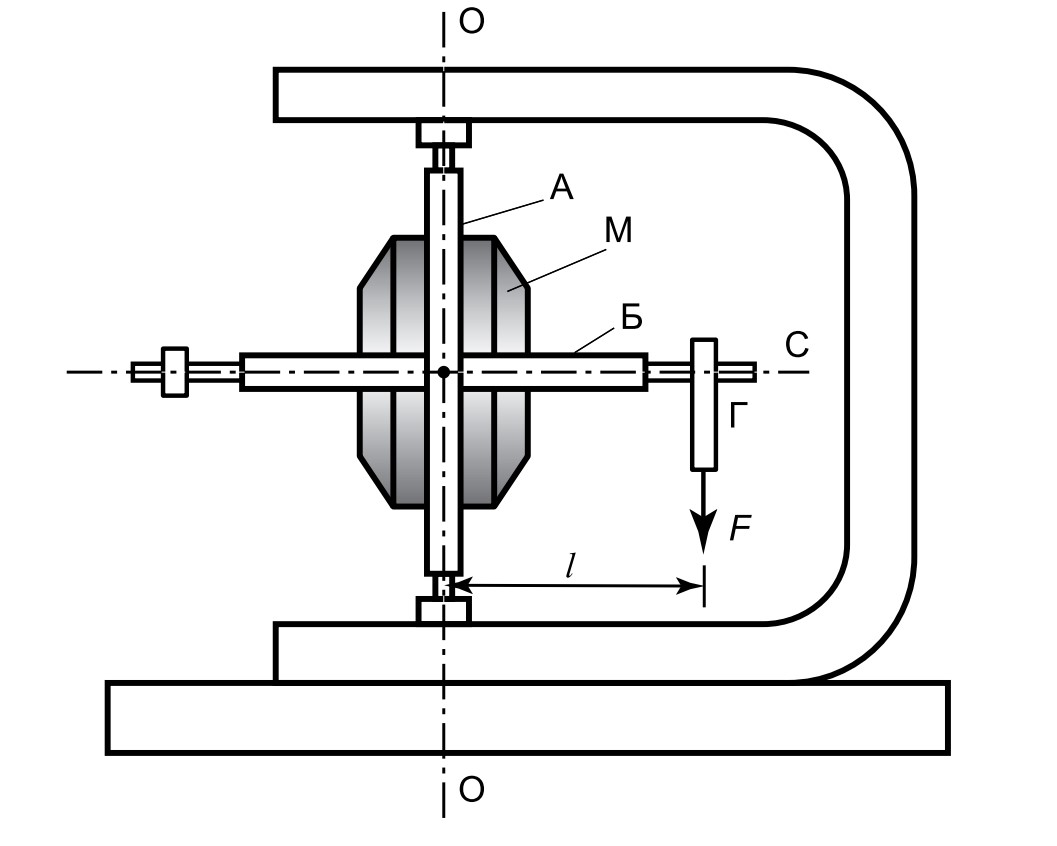
\includegraphics[width=0.8\textwidth]{fig1}
    \end{center}
    \caption{Схема экспериментальной установки гироскопа на кардановом подвесе, использованной в эксперименте.}
    \label{fig:1}
\end{figure}
\subsection{Определение моментов сил трения в различных осях}
Для определения момента силы трения $Mtr_1$ и $Mtr_2$ используем эффект прецессии гироскопа под действием небольшого момента силы тяжести, 
предполагая постоянство данных моментов, независимо от приложенного момента силы тяжести, так как его масса намного меньше массы гироскопа.
Из литературы\cite{LabBook} известны уравнения для связи главного момента импульса гироскопа $L$, момента силы тяжести $M$, 
момента силы трения $Mtr_2$ и угловой скорости прецессии $w$ относительно вертикальной оси:
\begin{equation}\label{eq:3}
    M = Lw - Mtr_2.
\end{equation}
Тогда измерив зависимость скорости прецессии от момента силы тяжести получим линейную зависимость с коэффициентом наклона $L$ и свободным членом
$-Mtr_2$.
Для определения момента силы трения $Mtr_1$ измерим горизонтальную прецессию $\alpha$ за время $t$ и, определив угловую скорость прецессии 
$W = \frac{\alpha}{t}$ относительно горизонтальной оси, оценим момент силы трения $Mtr_1$ с использованием ранее найденного $L$:
\begin{equation}\label{eq:4}
    Mtr_1 = LW.
\end{equation}
Для определения момента силы трения $Mtr_3$ измерено затухание частоты смены полярности обмотки $f$. Известно, что частота смены полярности обмотки $f$
зависит от угловой скорости вращения гироскопа $w$ на константу $Q$, $w = Qf$. Предполагая степенную зависимость момента силы трения $Mtr_3 = -\gamma w^n$
от угловой скорости вращения гироскопа $w$ получена связь первой производной $\frac{df}{dt}$ от частоты $f$ и $A = \frac{\gamma Q^{n-1}}{I}$:
\begin{equation}\label{eq:5}
    \frac{df}{dt} = -Af^n.
\end{equation}
Для нахождения степени $n$ прологарифмировано выражение \ref{eq:5}:
\begin{equation}\label{eq:6}
    \ln{-\frac{df}{dt}} = \ln{A} + n\ln{f}.
\end{equation}
Построив график $\ln{\frac{df}{dt}}$ от $\ln{f}$, определим значение $n$ в качестве коэффициента наклона.
После интегрирования выражения \ref{eq:4} получена связь частоты $f$ от времени $t$ и величину $p = 1 - n$:
\begin{equation}\label{eq:7}
    f^p/p = f_0^p/p - At
\end{equation}
Из графиков $\frac{f^p/p}{p}$ от $t$ получим $A$ в качестве коэффициента наклона и $f_0^p/p$ в качестве свободного члена. Получим зависимость 
для момента силы трения $Mtr_3$:
\begin{equation}\label{eq:8}
    Mtr_3 = -\gamma w^n = \frac{AI}{Q^{n-1}} w^n
\end{equation}
И тогда момент силы трения $Mtr_{3_0}$ выражается через $w_0$:
\begin{equation}\label{eq:9}
    Mtr_{3_0} = -\gamma w_0^n = \frac{AI}{Q^{n-1}} w_0^n
\end{equation}

\section{Результаты и их анализ}
\subsection{Нахождение моментов сил трения во внешних осях гироскопа}
Результаты измерения параметров эталонного цилиндра и вычисления момента инерции гироскопа представлены в приложении \ref{app_1}.
Для построения определения момента импульса гироскопа $L$ и момента силы трения $Mtr_2$ были измерены периоды прецессии гироскопа в зависимости от момента силы, 
приложенного к его главной оси. Изменение момента силы достигалось за счёт изменения плеча её приложении и массы груза, подвешенного 
на ось гироскопа. Полученные данные занесены в таблицу \ref{tab:1}. Построенная зависимость (Рис. \ref{fig:2}) момента силы от угловой скорости прецессии $M(w)$
оказалась линейной, что подтверждает корректность применимости модели гироскопа в данной задаче. Из выражения \ref{eq:3} найден момент импульса
гироскопа $L = (1.93 \pm 0.01)$~$\frac{\textrm{кг} \cdot \textrm{м}^2}{\textrm{с}}$ и момент силы трения 
$Mtr_2 = (3.4 \pm 0.7) \cdot 10^{-3}$~$\frac{\textrm{кг} \cdot \textrm{м}^2}{\textrm{с}}$.
\begin{figure}[H]
    \begin{center}
        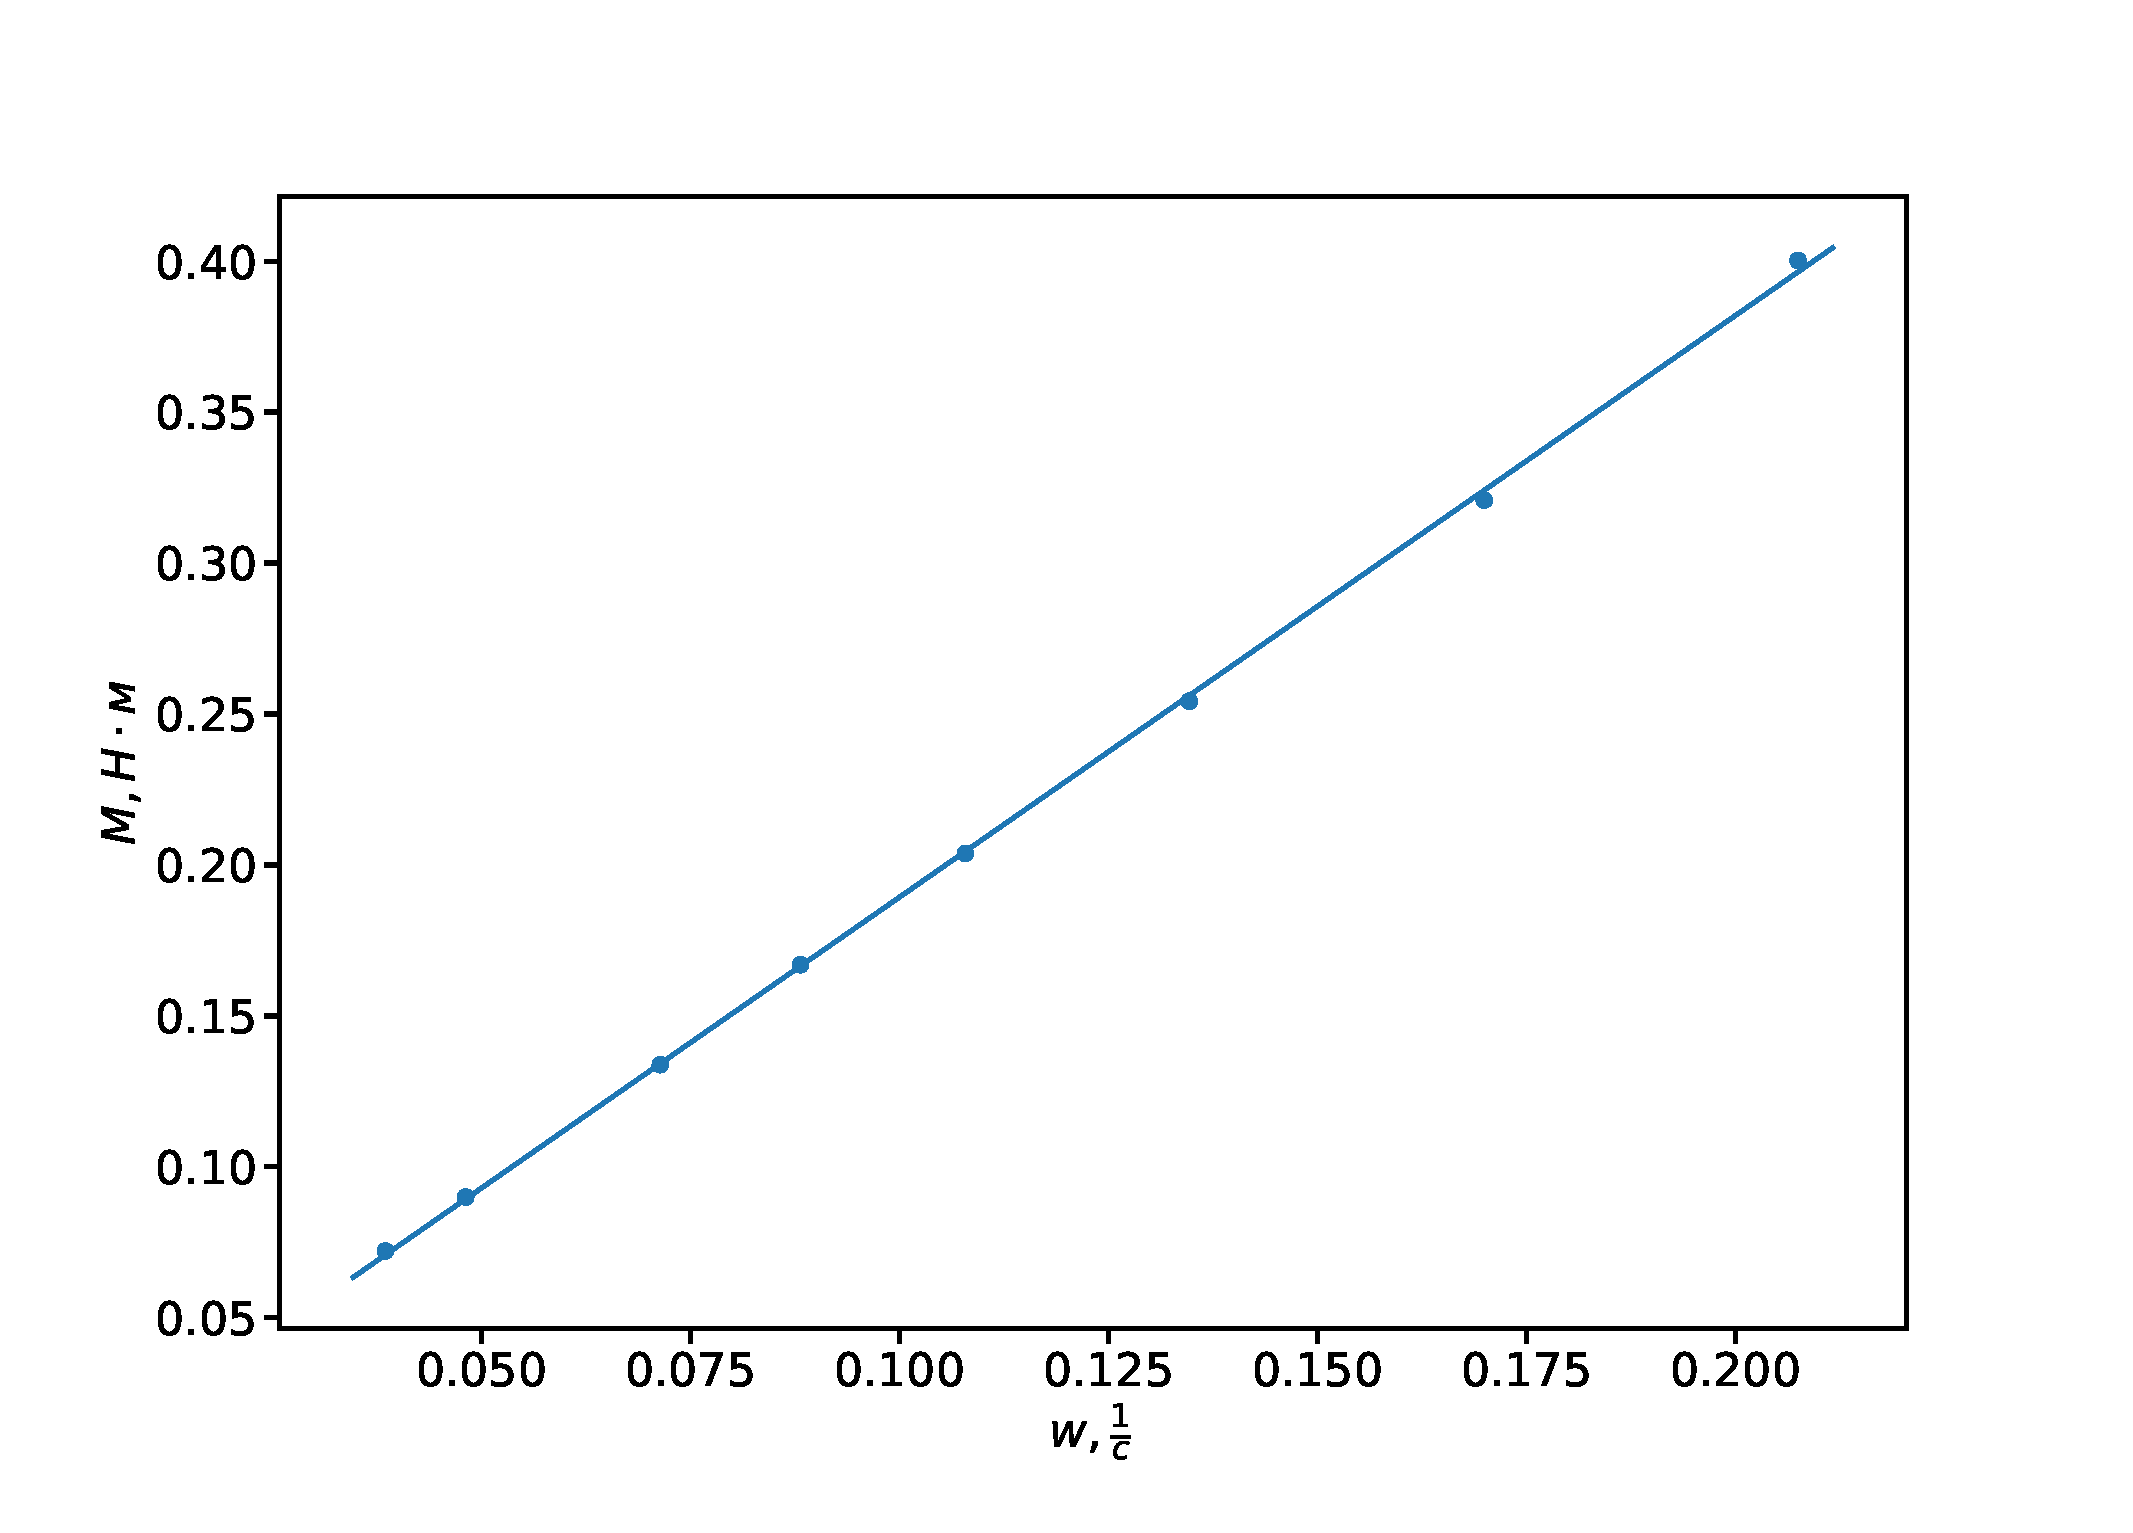
\includegraphics[width=0.8\textwidth]{1.eps}
    \end{center}
    \caption{Зависимость момента силы, приложенного к оси гироскопа, $M$ от угловой скорости прецессии оси $w$ в горизонтальной плоскости.}
    \label{fig:2}
\end{figure}
Для определения момента силы трения $Mtr_1$ была измерена угловая скорость прецессии в вертикальной плоскости $W$ (Таблица \ref{tab:1}).
Тогда из выражения \ref{eq:4} получено значение $Mtr_1 = (2.26 \pm 0.03) \cdot 10^{-3}$~$\frac{\textrm{кг} \cdot \textrm{м}^2}{\textrm{с}}$.

\subsection{Нахождение момента силы трения во внутренней оси гироскопа}
Для измерения частоты перемагничивания обмотки гироскопа $f$ использованы осциллограф и генератор переменного тока, 
на котором во время эксперимента подбиралась такая частота сигнала, чтобы на осциллографе получался эллипс. Данные измерения приведены в 
таблице~\ref{tab:2}. Из графика зависимости частоты перемагничивания обмотки гироскопа (Рис. \ref{fig:3}) от времени получено, что зависимость не является 
линейной, а значит момент силы трения зависит от частоты вращения гироскопа.
\begin{figure}[H]
    \begin{center}
        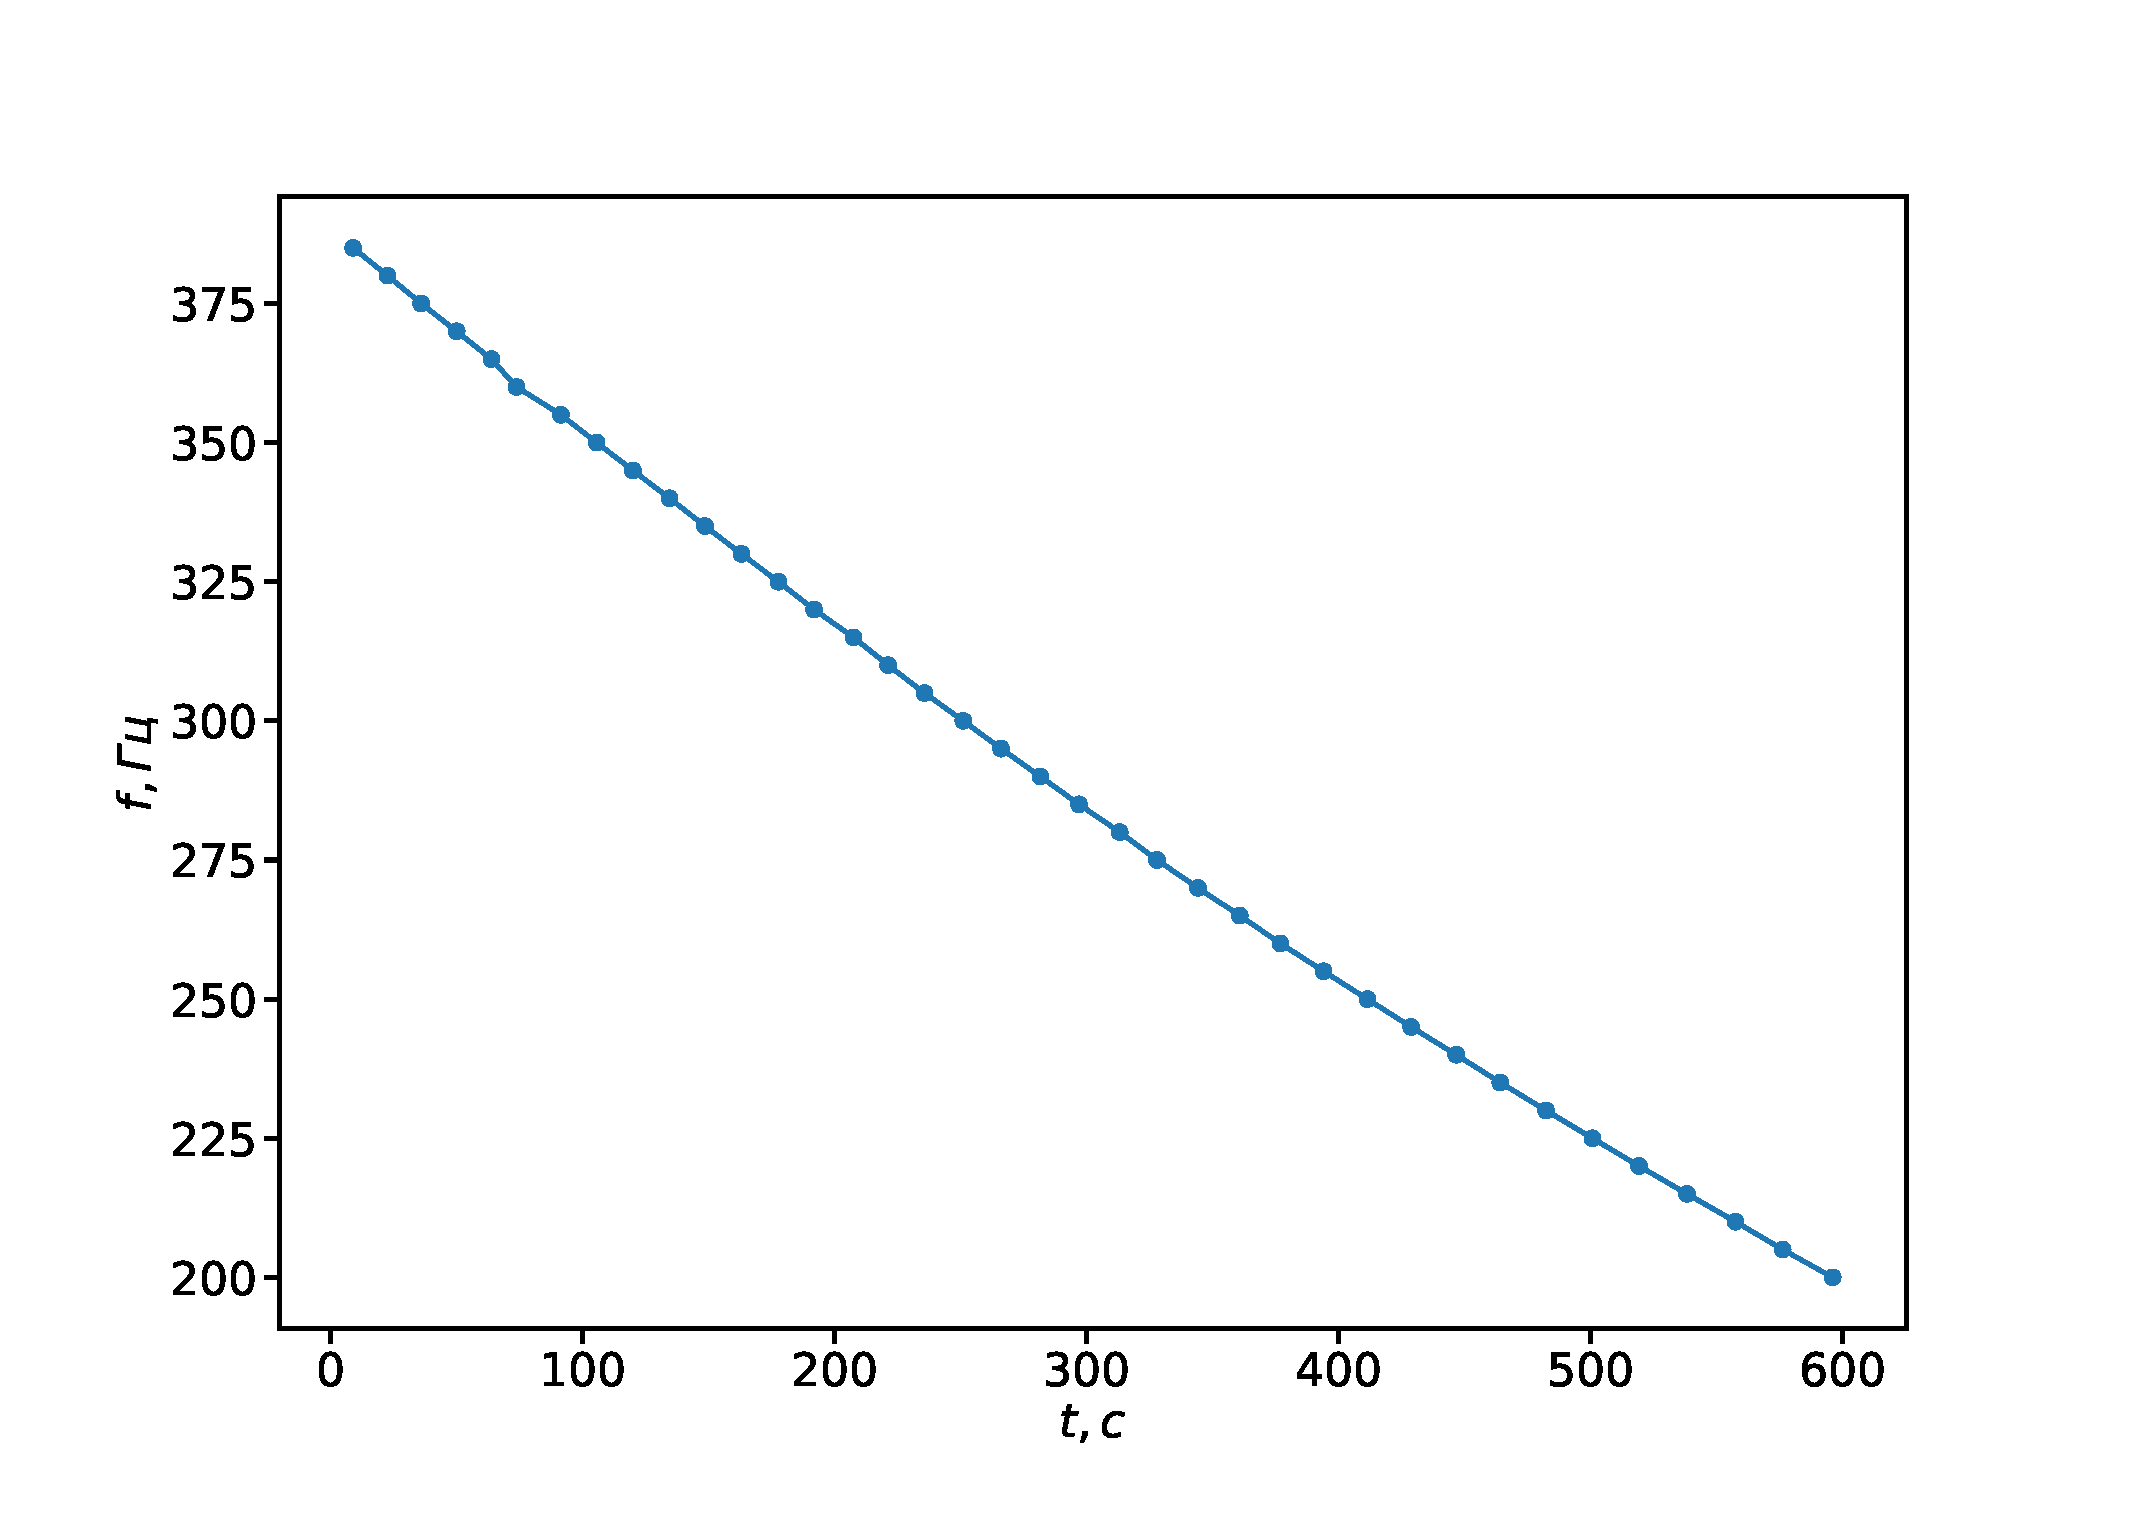
\includegraphics[width=0.8\textwidth]{2.eps}
    \end{center}
    \caption{Зависимость частоты перемагничивания обмотки гироскопа $f$ от времени измерения $t$.}
    \label{fig:3}
\end{figure}
Согласно методике \ref{eq:6}, предполагая зависимость момента силы трения $Mtr_3$ от частоты вращения $\omega$ степенной, построим график в логарифмическом
масштабе (Рис. \ref{fig:4}).
\begin{figure}[H]
    \begin{center}
        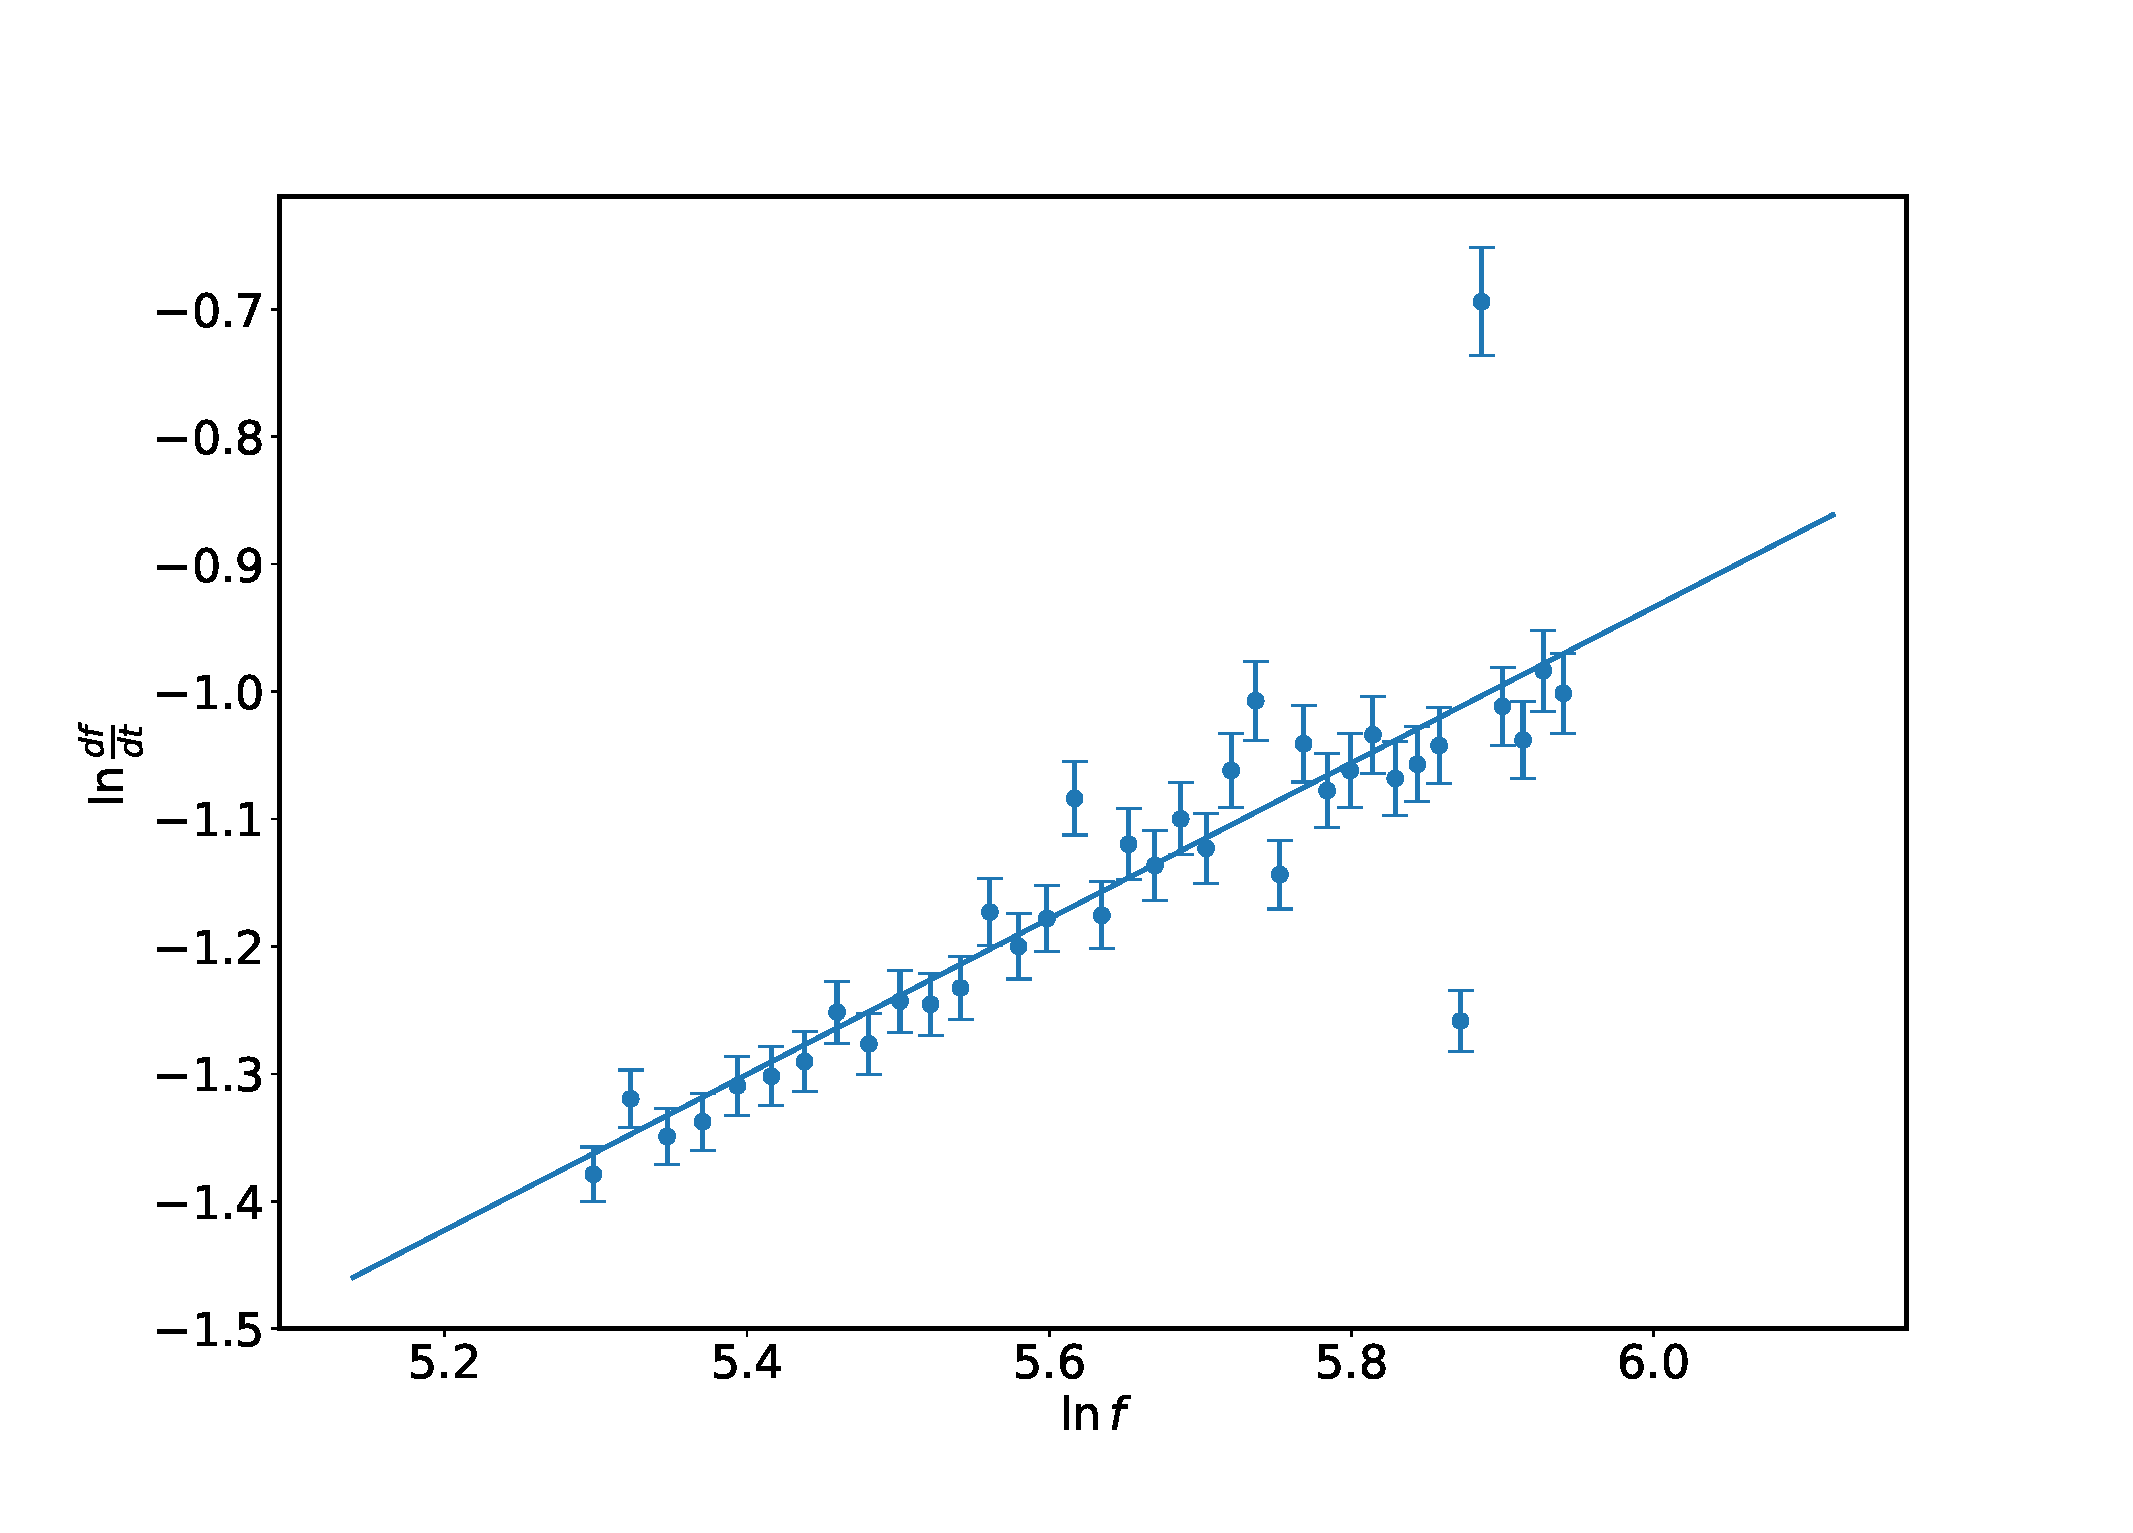
\includegraphics[width=0.8\textwidth]{3.eps}
    \end{center}
    \caption{Зависимость производной частоты перемагничивания обмотки гироскопа $\frac{df}{dt}$ от частоты перемагничивания обмотки $f$ 
    в логарифмическом масштабе.}
    \label{fig:4}
\end{figure}
Из графика следует, что зависимость \ref{eq:6} хорошо приближается линейной функцией с коэффициентом наклона $n = 0.61 \pm 0.07$. 
Для проверки правильности линеаризации исходной зависимости предложенной теорией был построен следующий график (Рис. \ref{fig:5}).
Из того, что полученный график хорошо приближается прямой можно сделать вывод о правильности предложенной гипотезы. А значит момент силы трения
в оси $Mtr_3$ зависит от частоты вращения $\omega$ степенным образом с показателем степени $n = 0.61$, что соответствует выражению \ref{eq:8}.
\begin{figure}[H]
    \begin{center}
        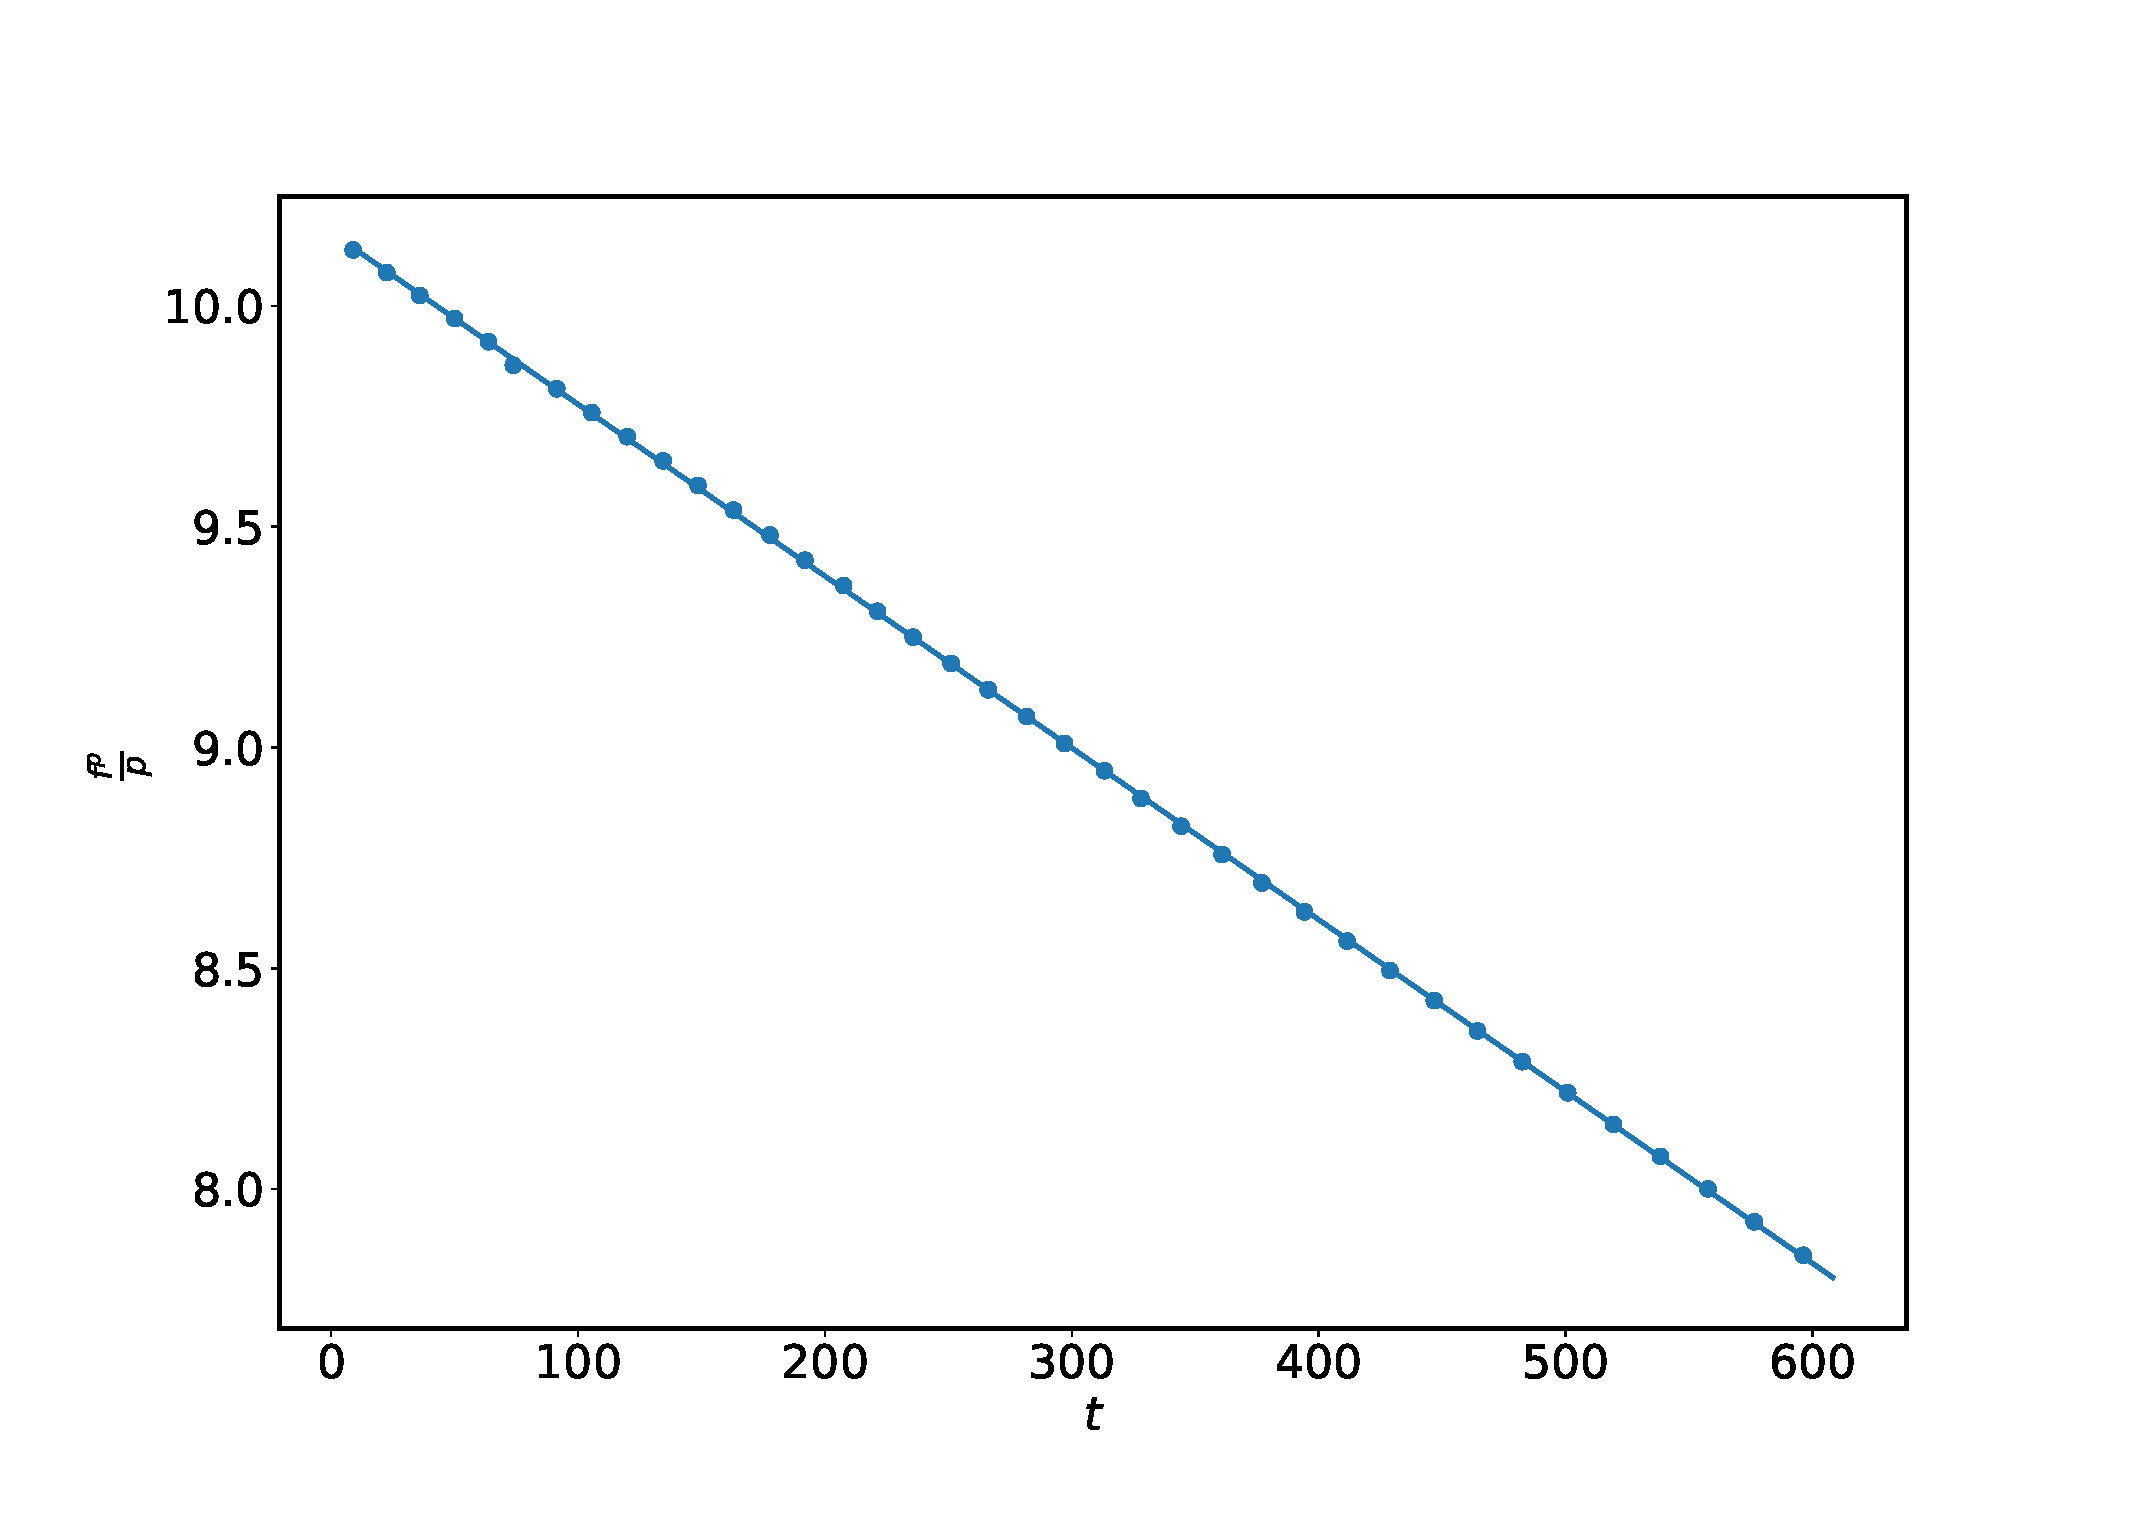
\includegraphics[width=0.8\textwidth]{4.eps}
    \end{center}
    \caption{Линеаризованная зависимость частоты перемагничивания обмотки гироскопа $f^p$, где $p = 1 - n$, $n$ - степень зависимости
    момента силы трения в оси от частоты вращения гироскопа, от времени измерения $t$.}
    \label{fig:5}
\end{figure}
Из графика \ref{fig:5} найдена начальная частота перемагничивания обмотки $f_0 = (388.9 \pm 0.2) \textrm{ Гц}$. Рассчитав начальную угловую скорость
вращения $\omega_0 = L/I = (1330 \pm 20)$~$\frac{1}{\textrm{с}}$, получено значение $Q = \frac{\omega_0}{f_0} = 3.42 \pm 0.05$.

Из графика \ref{fig:5} рассчитан коэффициент наклона $-A = (-3.892 \pm 0.004) \cdot 10^{-3}$~$\frac{1}{\textrm{с}^{2-n}}$
Тогда согласно выражению \ref{eq:8} получено $\gamma = (9.1 \pm 0.7) \cdot 10^{-6}$~$\textrm{кг}\cdot\textrm{м}^2\cdot\textrm{кг}^{n-2}$. 
Следовательно момент силы трения $Mtr_{3_0} = (12 \pm 1) \cdot 10^{-3}$~$\frac{\textrm{кг} \cdot \textrm{м}^2}{\textrm{с}}$.

\section{Выводы}
Моменты сил трения во внешних осях оказались равны $Mtr_1 = (2.26 \pm 0.03) \cdot 10^{-3}$~$\frac{\textrm{кг} \cdot \textrm{м}^2}{\textrm{с}}$ и 
$Mtr_2 = (3.4 \pm 0.7) \cdot 10^{-3}$~$\frac{\textrm{кг} \cdot \textrm{м}^2}{\textrm{с}}$. Зависимость момента силы трения во внутренней оси 
подчиняется закону $Mtr_3 = -\gamma w^n$, где $n = 0.61 \pm 0.07$, а $\gamma = (9.1 \pm 0.7) \cdot 10^{-6}$~$\textrm{м}^2\cdot\textrm{кг}^{n-1}$.

\section{Использованная литература}
\begin{thebibliography}{9}
    \bibitem{LabBook}
    Лабораторный практикум по общей физике, Том 1, под редакцией А. Д. Гладуна
\end{thebibliography}

\section{Приложения}
\subsection{Расчёт момента инерции гироскопа} \label{app_1}
Масса эталонного цилиндра составила $M = (1616.7 \pm 0.1) \textrm{ г}$, а радиус составил $R = (3.800 \pm 0.001) \textrm{ см}$.
тогда момент инерции цилиндра равняется $I_0 = (2.334 \pm 0.003) \cdot 10^{-3} \textrm{ кг} \cdot \textrm{м}^2$. Измерены периоды крутильных колебаний 
гироскопа $T = (3.150 \pm 0.015)$ c и цилиндра $T = (4.000 \pm 0.015)$ c. Тогда из соотношения \ref{eq:1} получим 
$I = (1.44 \pm 0.02) \cdot 10^{-3} \textrm{ кг} \cdot \textrm{м}^2$.
\subsection{Данные результатов измерения периода прецессии гироскопа} \label{app_2}
\begin{table}[H]
    \centering
    \begin{tabular}{|l|l|l|l|l|l|l|l|l|}
        \hline
        m, г  & l, см & M, кг$\cdot$м & h, см & $\alpha$    & n & t, с   & w, $\frac{1}{\textrm{с}}$ & W, $\frac{1}{\textrm{с}}$ \\ 
        \hline
        337,5 & 121   & 0,4002075     & 18    & 14,20556517 & 7 & 211,95 & 0,207512607               & 0,001169775               \\
        337,5 & 97    & 0,3208275     & 18    & 14,20556517 & 6 & 221,78 & 0,169984272               & 0,001117927               \\ 
        214,4 & 121   & 0,25423552    & 17,5  & 9,470376779 & 3 & 139,95 & 0,134687788               & 0,001181059               \\
        214,4 & 97    & 0,20380864    & 17,5  & 9,470376779 & 2 & 116,45 & 0,107912156               & 0,001419401               \\ 
        140,8 & 121   & 0,16696064    & 18    & 14,20556517 & 3 & 213,72 & 0,088197436               & 0,001160087               \\ 
        140,8 & 97    & 0,13384448    & 18,5  & 18,94075356 & 3 & 263,92 & 0,071421476               & 0,001252571               \\ 
        75,9  & 121   & 0,09000222    & 18    & 14,20556517 & 2 & 261,02 & 0,048143325               & 0,000949865               \\ 
        75,9  & 97    & 0,07215054    & 18,7  & 20,83482891 & 2 & 326,13 & 0,038531784               & 0,001115004               \\ 
        \hline
    \end{tabular}
    
    \caption{Данные результатов измерения прецессии гироскопа под действием момента силы тяжести в двух осях. $m$ - масса подвешенного груза,
        $l$ - длина плеча подвеса, $M$ - рассчитанный момент импульса, $h$ - начальная высота крайней точки оси гироскопа, $\alpha$ - перемещение 
        крайней точки оси гироскопа за время измерения, $n$ - количество оборотов, совершённое осью гироскопа, $t$ - время измерения, 
        $w$ - рассчитанная угловая скорость прецессии в горизонтальном направлении, $W$ - рассчитанная угловая скорость прецессии в вертикальном направлении}
    \label{tab:1}
\end{table}

\subsection{Данные результатов измерения замедления вращения гироскопа} \label{app_3}
\begin{table}[H]
    \centering
    \begin{tabular}{|l|l|}
        \hline
        t, с      & $f$, Гц   \\ 
        \hline
        8,92   & 385 \\
        22,53  & 380 \\ 
        35,9   & 375 \\ 
        50,02  & 370 \\ 
        63,77  & 365 \\ 
        73,78  & 360 \\ 
        91,38  & 355 \\ 
        105,56 & 350 \\
        119,95 & 345 \\
        134,5  & 340 \\ 
        148,56 & 335 \\
        163,02 & 330 \\
        177,71 & 325 \\
        191,87 & 320 \\
        207,56 & 315 \\
        221,25 & 310 \\
        235,71 & 305 \\
        251,08 & 300 \\
        266,1  & 295 \\ 
        281,68 & 290 \\ 
        297    & 285 \\ 
        313,2  & 280 \\ 
        327,98 & 275 \\
        344,22 & 270 \\
        360,82 & 265 \\
        376,98 & 260 \\
        394,13 & 255 \\
        411,5  & 250 \\ 
        428,83 & 245 \\
        446,75 & 240 \\
        464,23 & 235 \\
        482,4  & 230 \\ 
        500,78 & 225 \\
        519,3  & 220 \\ 
        538,35 & 215 \\
        557,62 & 210 \\
        576,33 & 205 \\
        596,18 & 200 \\
        \hline
    \end{tabular}
    
    \caption{Данные результатов измерения замедления вращения гироскопа. $t$ - время, прошедшее с момента отключения питания гироскопа, 
    $f$ - частота перемагничивания обмотки, измеренная при помощи осциллографа.}
    \label{tab:2}
\end{table}
\subsection{Метод наименьших квадратов} \label{app_4}
$$y = a + bx$$
Формула для расчёта коэффициентов $a$ и $b$:
$$b = \frac{\overline{xy} - \overline{x}\overline{y}}{\overline{x^2} - \overline{x}^2}$$
$$a = \overline{y} - b\overline{x}$$
Погрешности:
$$\sigma_b \approx \frac{1}{\sqrt{n}}\sqrt{\frac{\overline{y^2} - \overline{y}^2}{\overline{x^2} - \overline{x}^2} - b^2}$$
$$\sigma_a \approx \sigma_b \sqrt{\overline{x^2} - \overline{x}^2}$$


\subsection{Расчёт погрешностей} \label{app_5}
$$\sigma_{I_0} = I_0\sqrt{\left[\left(\frac{\sigma_M}{M}\right)^2 + \left(2\frac{\sigma_R}{R}\right)^2\right]}$$
$$\sigma_{I} = I\sqrt{\left[\left(\frac{\sigma_{I_0}}{I_0}\right)^2 + \left(2\frac{\sigma_T}{T}\right)^2 + \left(2\frac{\sigma_{T_0}}{T_0}\right)^2\right]}$$
Для нахождения погрешностей величин, рассчитанных из графика используем формулу случайной погрешности из приложения \ref{app_5}. Будем обозначать
случайную погрешность величины $\theta$ как $\sigma_{\theta_1}$, а приборную как $\sigma_{\theta_2}$ 
$$\sigma_L = \sqrt{\left[\left(\sigma_{L_1}\right)^2 + L^2 \cdot max\left(\left(\frac{\sigma_w}{w}\right)^2 + \left(\frac{\sigma_M}{M}\right)^2\right)\right]}$$
$$\sigma_{Mtr_2} = \sqrt{\left[\left(\sigma_{{Mtr_2}_1}\right)^2 + Mtr_2^2 \cdot max\left(\left(\frac{\sigma_w}{w}\right)^2 + \left(\frac{\sigma_M}{M}\right)^2\right)\right]}$$
Погрешность $\sigma_{{Mtr_1}_1}$ найдём как среднеквадратичное отклонение среднего из выборки.
$$\sigma_{Mtr_1} = \sqrt{\left[\left(\sigma_{{Mtr_1}_1}\right)^2 + Mtr_1^2 \cdot max\left(\left(\frac{\sigma_W}{W}\right)^2 + \left(\frac{\sigma_L}{L}\right)^2\right)\right]}$$
$$\sigma_n = \sqrt{\left[\left(\sigma_{n_1}\right)^2 + n^2 \cdot max\left(\left(\frac{\sigma_{\frac{df}{dt}}}{\frac{df}{dt}}\right)^2\right)\right]}$$
$$\sigma_p = \sigma_{1-n} = \sigma_n$$ 
\end{document}